\section{Visualisierung des Co-Autor-Graphen}
Um Informationen �ber einzelne Autoren und deren Communities aus dem Co-Autor-Graphen gewinnen zu k�nnen muss der Co-Author-Graph auf geeignete Art visualisiert werden. Daher wird versucht folgende Frage zu beantworten: 

 \begin{center}
\textit{L�sst sich das Umfeld eines Autors im Co-Autor-Graphen und seine Community visualisieren?}
\end{center}
 Der in der Neo4j-Datenbank gespeicherte Graph kann zwar �ber die in Neo4j eingebauten Bordmittel bereits teilweise visualisiert werden, allerdings funktioniert die Visualisierung bei dieser Datenmenge nur stark eingeschr�nkt. Vor allem die Tatsache, dass bei dieser Art von Visualisierung der jeweils betrachtete Teil des Graphen dynamisch aus der Datenbank gelesen werden muss, schr�nkt den Gesamtprozess stark ein. \\
 Daher wird mit einem neuen Modul f�r die in Abschnitt \ref{randbendingingen} beschriebene Applikation der gesamte Graph mit allen enthaltenen Knoten in eine statische \acs{HTML}-Struktur exportiert. 
 \subsection{Visualisierung des Graphen mit \acs{HTML}}
  Abbildung \ref{img:web} zeigt eine der durch die vorher beschriebe Methode entstandenen \acs{HTML}-Seiten. Die einzelnen Autoren untereinander enthalten \acs{HTML}-Verlinkungen zu allen Nachbarautoren und der Communities (pro jede Hierarchieebene eine) denen sie angeh�ren. 
 \begin{center}
					\hpic{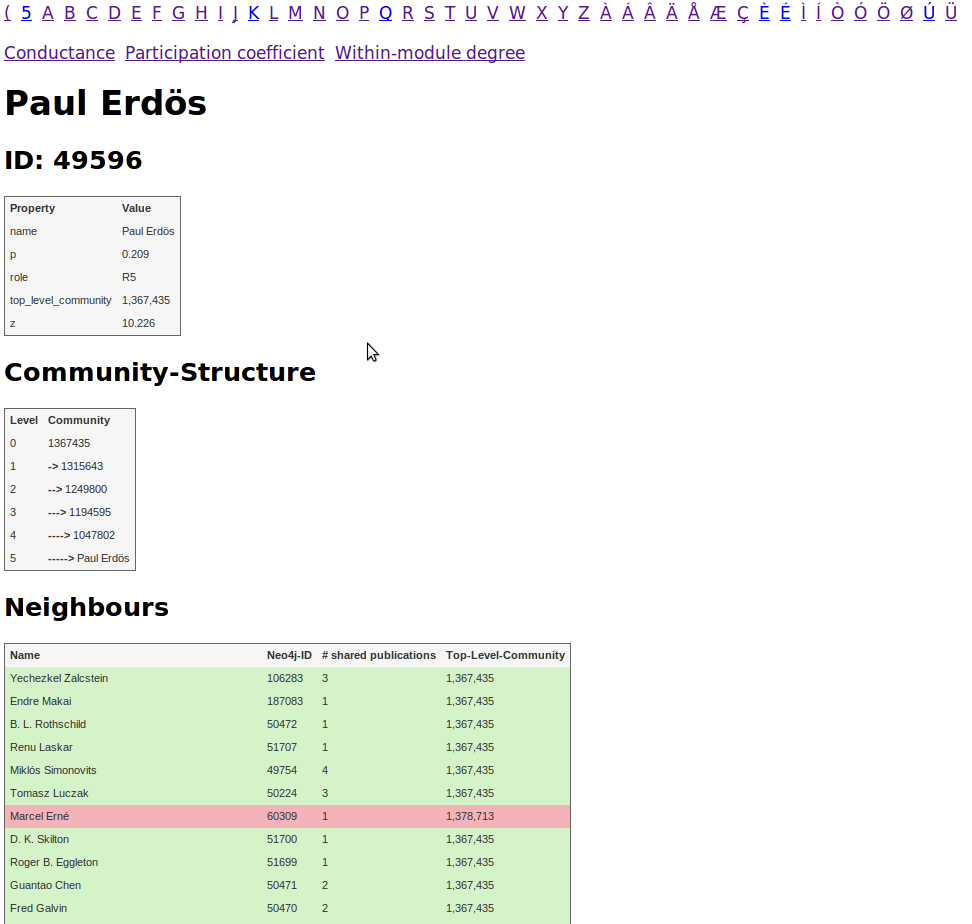
\includegraphics[width=1\textwidth]{images/web}
					} \newcaption{HTML-Darstellung vom Autorknoten Paul Erd�s}
					\label{img:web}
	\end{center}
  Diese Art der Visualisierung verhindert, dass der Graph bei Betrachtung dynamisch aus der Datenbank geladen werden muss, da dies bereits zum Zeitpunkt des \acs{HTML}-Exports geschieht. Auf diese Art kann das Umfeld eines Autors effizient und schnell durchsucht werden. Durch einen alphabetischen Index k�nnen Autoren schnell gefunden und analysiert werden. 
% { Methoden }

% { Ergebnisse }

% { Diskussion }